\documentclass[../index.tex]{subfiles}

\begin{document}
Для того аби зрозуміти як працюють біржі основані на механізмах АММ, розглянемо
існуючий, загальноприйнятий варіант імплементації на впорядкованих книжках,
записах~\cite{MERTENS2003433} (від англ. \textit{``order books''}).

\begin{definition}
  \textbf{Впорядкована книжка} --- це списки запитів на купівлю та продаж активів, що
  відображається у вигляді впорядкованої таблиці з пропонованими цінами та
  об'ємами.
\end{definition}

У випадках коли система, що впорядковує таблиці, знаходить співпадіння у
таблицях по ціні та об'єму, стається обмін і обидва запити в обох таблицях
виконуються та видаляються з них. Прикладом таких впорядкових таблиць є
табл.~\ref{table:order-book}, де виділений рядок є співпадінням котрий система
обробить автоматично.

\begin{table}[H]
  \centering
  \begin{tabular}{ c | c }
    Об'єм & Ціна \\
    \hline \hline
    1 & 10,0 \\
    \rowcolor{green} 2 & 9,95 \\
    3 & 9,87 \\
    4 & 9,71
  \end{tabular}
  \quad
  \begin{tabular}{ c | c }
    Ціна & Об'єм \\
    \hline \hline
    10,1 & 1 \\
    \rowcolor{green} 9,95 & 2 \\
    10,3 & 3 \\
    10,4 & 4
  \end{tabular}

  \caption{Таблиці на купівлю (зліва) та продаж (справа)}\label{table:order-book}
\end{table}

У протиставлення до цього АММ визначає формулу $\Phi(\Delta x, \Delta y)$ обміну (трейду чи
торгу) над $\Delta x \in \mathbb{R}$ --- вхідний об'єм, що користувач пропонує віддати, та
$\Delta y \in \mathbb{R}$ --- вихідний об'єм іншої валюти, що користувач пропонує отримати. У
випадку, коли формула $\Phi$ для $\Delta x$ та $\Delta y$ не справджується, то обмін не
стається.

Для задовільнення пропозицій обмінів, біржа оперує об'ємами цих валют. У
випадку, коли для запропонованих користувачем $\Delta x > 0$, $\Delta y < 0$ значення
$\Delta x$ додається до резервів першої валюти, а $\Delta y$ віднімається від другої
рис.~\ref{fig:amm-exchange}.

\begin{figure}[ht]
  \centering
  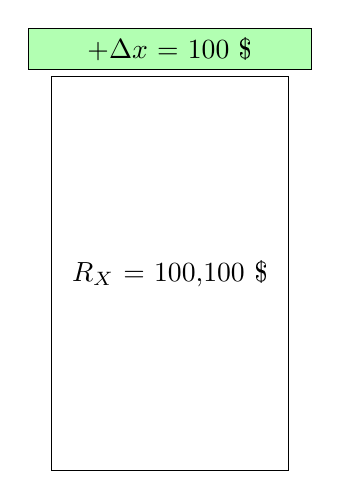
\begin{tikzpicture}
    \node[rectangle,
    fill = white,
    minimum width = 3cm,
    minimum height = 5cm,
    draw] (r) at (0,0) { $R_{X}$ = 100,100 \$};
    \node[rectangle,
    fill = green!30!white,
    minimum width = 3.6cm,
    minimum height = 0.5cm,
    draw] (r) at (0,2.85) { $+ \Delta x$ = 100 \$};
  \end{tikzpicture}
  \quad
  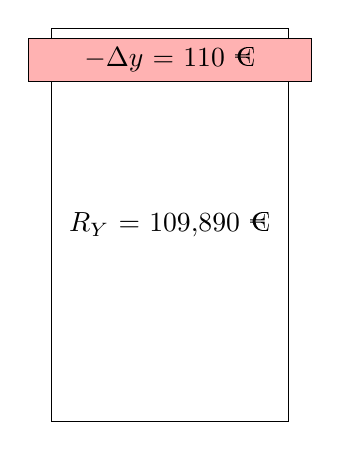
\begin{tikzpicture}
    \node[rectangle,
    fill = white,
    minimum width = 3cm,
    minimum height = 5cm,
    draw] (r) at
    (0,0) { $R_{Y}$ = 109,890 €};
    \node[rectangle,
    fill = red!30!white,
    minimum width = 3.6cm,
    minimum height = 0.5cm,
    draw] (r) at (0,2.1) { $- \Delta y$ = 110 €};
  \end{tikzpicture}
  \caption{\label{fig:amm-exchange} $R_{X}$ --- резерви валюти $X$ = USD, $R_{Y}$ ---
    резерви валюти $Y$ = EUR}
\end{figure}

АММ поділяється на різні види та групи, у випадку ММКФ умовою є те, що значення
деякої функції $\varphi$ від резервів до обміну має дорівнювати значенню після обміну
і формула визначається наступним чином:

\begin{equation*}
\varphi(R_{X} + \Delta x, R_{Y} - \Delta y) = \varphi(R_{X}, R_{Y})
\end{equation*}

У випадку ММКД зі вступу:

\begin{equation*}
R_{X} \cdot R_{Y} = (R_{X} + \Delta x) \cdot (R_{Y} - \Delta y)
\end{equation*}

Залежність між $\Delta x$ та $\Delta y$ визначається через функцію обміну, що і
пропонується розглянути у наступному розділі.

\end{document}
